\documentclass[a4paper,12pt]{article}
\usepackage{graphicx}
\usepackage{amsmath}
\usepackage{tkz-euclide}
\usepackage{booktabs}
\title{Assignment-5\\ Latex Report}
\author{Fuzayil Bin Afzal Mir}
\date{18/01/2021}
\begin{document}
	\maketitle
	
	
	\newpage
	\begin{itemize}
	    \item \Large\textbf{Exercise 2.11}
	\end{itemize}
	\section{Draw an equilateral triangle of side 5.5.}\\
    	
\subsection{Solution} \\
  Let $\triangle$ABC be an equilateral triangle of side 5.5\\
  Since ,In an equilateral triangle all sides are equal to each other and also each angle is equal to 60$^{\circ}$.\\
  Therefore,\\
  
  a=b=c=5.5 \hspace{2cm}{and} \hspace{4cm}{$\angle$A=$\angle$B=$\angle$C=60$^{\circ}$ }\\
  
\textbf{Equilateral triangle ABC}\\



\begin{tikzpicture}[scale=1]
    \coordinate[label=right:$C$] (C) at (5.5,0);
    \coordinate[label=left:$B$] (B) at (0,0);
    \coordinate[label=above:$A$] (A) at (2.75,4.75);
    
    \draw (A)--node[above] {$\textrm{c}$}
    (B)--node[above] {$\textrm{a}$}
    (C)--node[above] {$\textrm{b}$}(A);
    \tkzMarkAngle[fill=green!15,size=0.5](B,A,C);
    
    \tkzMarkAngle[fill=pink!10,size=0.5](A,C,B);
    
     \tkzMarkAngle[fill=green!30,size=0.5](C,B,A);
     
    \end{tikzpicture}\\$$$$\\
    
\textbf{\underline{Note:}} {Figure generated using latex}\\

\subsection{Figure of $\triangle$ABC,}
\begin{figure}[htp]
    \centering
    \includegraphics[width=10cm]{2.11.png}
    \caption{Generated using python}
    \label{fig:2}
\end{figure}
 \newpage
 \begin{itemize}
	    \item \Large\textbf{Exercise 2.12}
	\end{itemize}
	\section{Draw a $\triangle$PQR with PQ=4,QR=3.5 and PR=4.What type of triangle is this?}\\
    	
\subsection{Solution} \\
  In the given $\triangle$PQR, \\
   PQ=4,QR=3.5 and PR=4\\
   or we can say,\\
   PQ=r=4,\\QR=p=3.5\\ and\\ PR=q=4\\
  
   In the given $\triangle$PQR, two sides are of equal length.(i.e PQ=PR=4) \hspace{0.5cm}{or} \hspace{0.5cm}{(r=q=4)} which is the property of an isosceles triangle.\\
  
  Therefore, the given $\triangle$PQR is an isosceles triangle.\\
   \\
  
\textbf{Figure of triangle PQR}

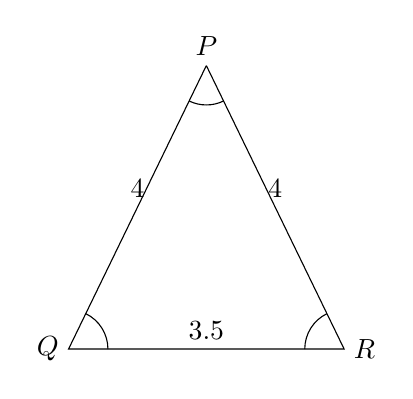
\begin{tikzpicture}[scale=1]
    \coordinate[label=right:$R$] (R) at (3.5,0);
    \coordinate[label=left:$Q$] (Q) at (0,0);
    \coordinate[label=above:$P$] (P) at (1.75,3.6);
    
    \draw (P)--node[above] {$\textrm{4}$}
    (Q)--node[above] {$\textrm{3.5}$}
    (R)--node[above] {$\textrm{4}$}(P);
    \tkzMarkAngle[fill=green!15,size=0.5](Q,P,R);
    
    \tkzMarkAngle[fill=pink!10,size=0.5](P,R,Q);
    
     \tkzMarkAngle[fill=green!30,size=0.5](R,Q,P);
     
    \end{tikzpicture}\\
    \textbf{\underline{Note:}} {Figure generated using latex.}\\$$$$\\

\subsection{Figure of $\triangle$PQR}
\begin{figure}[htp]
    \centering
    \includegraphics[width=10cm]{2.12.png}
    \caption{Generated using python}
    \label{fig:2}
\end{figure}
























\end{document}


